\documentclass[14pt]{extbook}
\usepackage{multicol, enumerate, enumitem, hyperref, color, soul, setspace, parskip, fancyhdr} %General Packages
\usepackage{amssymb, amsthm, amsmath, latexsym, units, mathtools} %Math Packages
\everymath{\displaystyle} %All math in Display Style
% Packages with additional options
\usepackage[headsep=0.5cm,headheight=12pt, left=1 in,right= 1 in,top= 1 in,bottom= 1 in]{geometry}
\usepackage[usenames,dvipsnames]{xcolor}
\usepackage{dashrule}  % Package to use the command below to create lines between items
\newcommand{\litem}[1]{\item#1\hspace*{-1cm}\rule{\textwidth}{0.4pt}}
\pagestyle{fancy}
\lhead{Progress Quiz 7}
\chead{}
\rhead{Version ALL}
\lfoot{3510-5252}
\cfoot{}
\rfoot{Summer C 2021}
\begin{document}

\begin{enumerate}
\litem{
Choose the equation of the function graphed below.
\begin{center}
    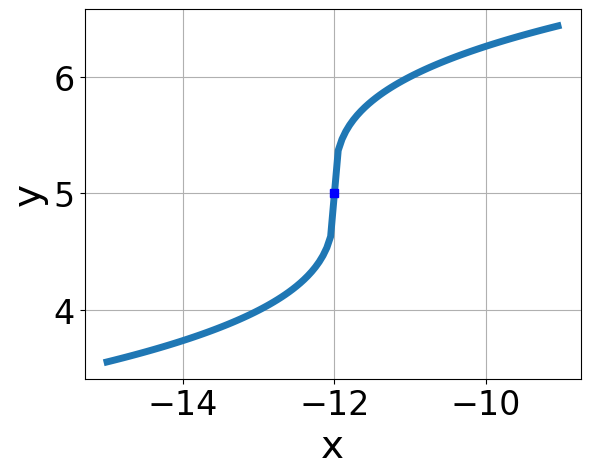
\includegraphics[width=0.5\textwidth]{../Figures/radicalGraphToEquationCopyA.png}
\end{center}
\begin{enumerate}[label=\Alph*.]
\item \( f(x) = - \sqrt[3]{x - 12} + 5 \)
\item \( f(x) = - \sqrt[3]{x + 12} + 5 \)
\item \( f(x) = \sqrt[3]{x - 12} + 5 \)
\item \( f(x) = \sqrt[3]{x + 12} + 5 \)
\item \( \text{None of the above} \)

\end{enumerate} }
\litem{
Choose the graph of the equation below.\[ f(x) = \sqrt{x + 10} + 4 \]\begin{enumerate}[label=\Alph*.]
\begin{multicols}{2}\item 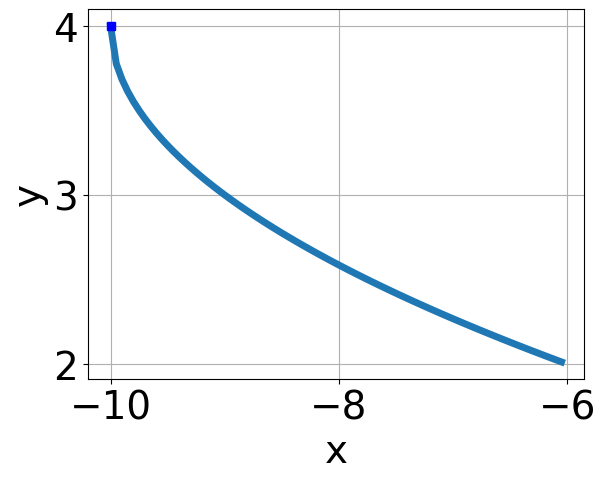
\includegraphics[width = 0.3\textwidth]{../Figures/radicalEquationToGraphAA.png}\item 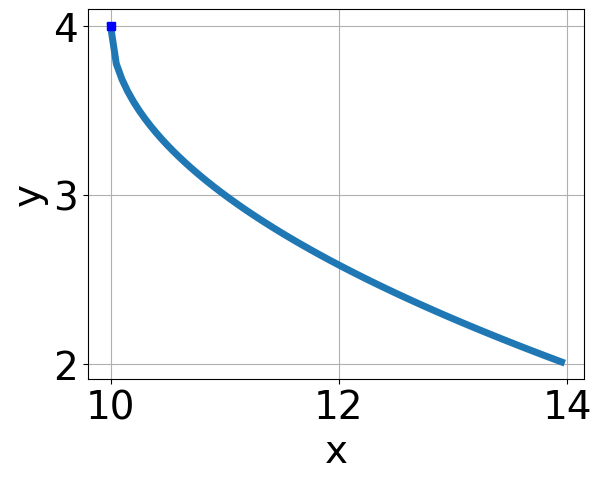
\includegraphics[width = 0.3\textwidth]{../Figures/radicalEquationToGraphBA.png}\item 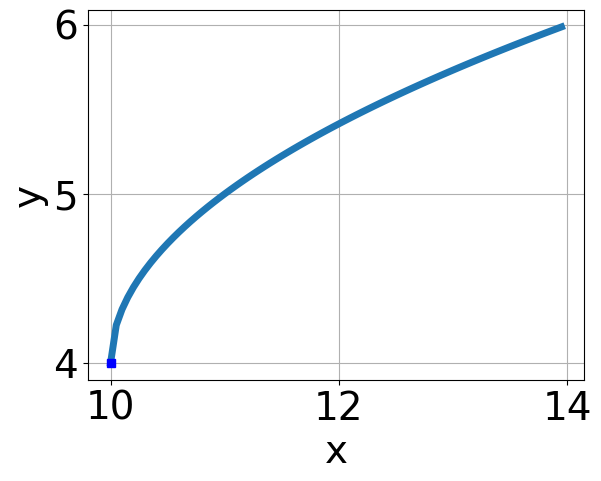
\includegraphics[width = 0.3\textwidth]{../Figures/radicalEquationToGraphCA.png}\item 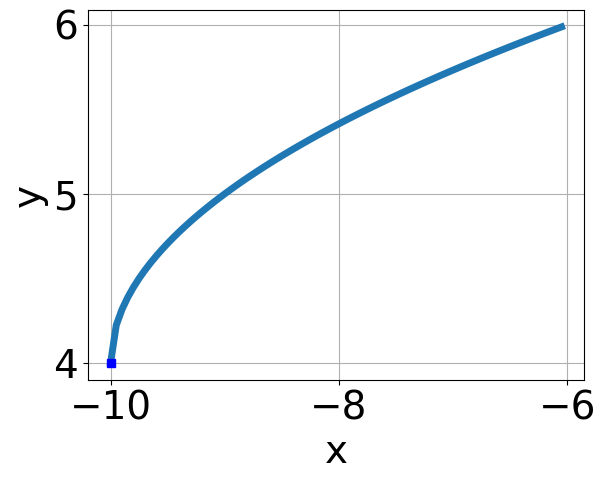
\includegraphics[width = 0.3\textwidth]{../Figures/radicalEquationToGraphDA.png}\end{multicols}\item None of the above.
\end{enumerate} }
\litem{
Solve the radical equation below. Then, choose the interval(s) that the solution(s) belongs to.\[ \sqrt{-36 x^2 - 12} - \sqrt{-42 x} = 0 \]\begin{enumerate}[label=\Alph*.]
\item \( x \in [0.2,0.59] \)
\item \( \text{All solutions lead to invalid or complex values in the equation.} \)
\item \( x_1 \in [-0.62, -0.24] \text{ and } x_2 \in [-2.67,0.33] \)
\item \( x_1 \in [0.2, 0.59] \text{ and } x_2 \in [-0.33,2.67] \)
\item \( x \in [0.66,1.01] \)

\end{enumerate} }
\litem{
Choose the equation of the function graphed below.
\begin{center}
    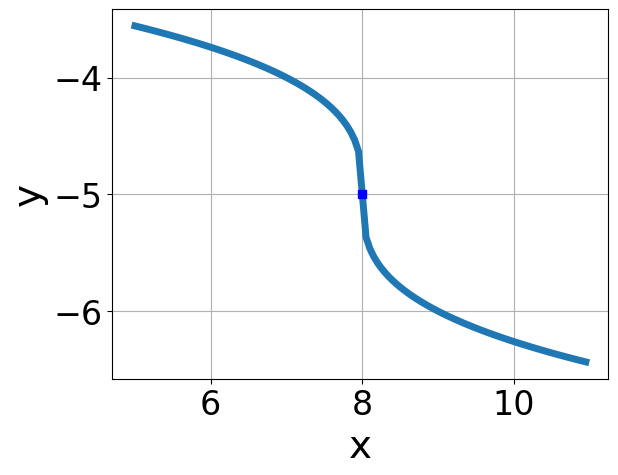
\includegraphics[width=0.5\textwidth]{../Figures/radicalGraphToEquationA.png}
\end{center}
\begin{enumerate}[label=\Alph*.]
\item \( f(x) = - \sqrt{x - 8} - 5 \)
\item \( f(x) = \sqrt{x - 8} - 5 \)
\item \( f(x) = - \sqrt{x + 8} - 5 \)
\item \( f(x) = \sqrt{x + 8} - 5 \)
\item \( \text{None of the above} \)

\end{enumerate} }
\litem{
Solve the radical equation below. Then, choose the interval(s) that the solution(s) belongs to.\[ \sqrt{56 x^2 + 15} - \sqrt{59 x} = 0 \]\begin{enumerate}[label=\Alph*.]
\item \( x_1 \in [-0.77, -0.42] \text{ and } x_2 \in [-1.17,0.14] \)
\item \( \text{All solutions lead to invalid or complex values in the equation.} \)
\item \( x_1 \in [0.41, 0.43] \text{ and } x_2 \in [-0.14,1.56] \)
\item \( x \in [0.58,0.79] \)
\item \( x \in [0.41,0.43] \)

\end{enumerate} }
\litem{
Solve the radical equation below. Then, choose the interval(s) that the solution(s) belongs to.\[ \sqrt{2 x + 8} - \sqrt{7 x - 5} = 0 \]\begin{enumerate}[label=\Alph*.]
\item \( x_1 \in [-4.6, -3.8] \text{ and } x_2 \in [-0.1,2.1] \)
\item \( \text{All solutions lead to invalid or complex values in the equation.} \)
\item \( x \in [0,0.9] \)
\item \( x_1 \in [-4.6, -3.8] \text{ and } x_2 \in [1.7,5] \)
\item \( x \in [1.8,2.9] \)

\end{enumerate} }
\litem{
What is the domain of the function below?\[ f(x) = \sqrt[8]{4 x - 3} \]\begin{enumerate}[label=\Alph*.]
\item \( (-\infty, a], \text{where } a \in [1.2, 1.4] \)
\item \( [a, \infty), \text{ where } a \in [0.51, 1.04] \)
\item \( [a, \infty), \text{where } a \in [0.76, 2.39] \)
\item \( (-\infty, \infty) \)
\item \( (-\infty, a], \text{where } a \in [-1.6, 1.2] \)

\end{enumerate} }
\litem{
Choose the graph of the equation below.\[ f(x) = - \sqrt{x + 14} - 7 \]\begin{enumerate}[label=\Alph*.]
\begin{multicols}{2}\item 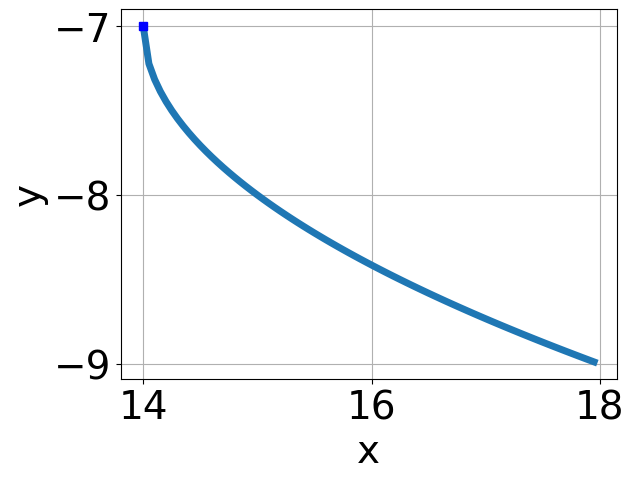
\includegraphics[width = 0.3\textwidth]{../Figures/radicalEquationToGraphCopyAA.png}\item 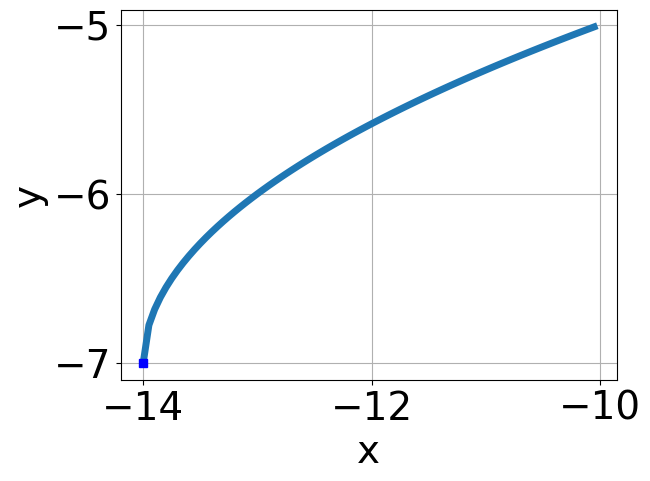
\includegraphics[width = 0.3\textwidth]{../Figures/radicalEquationToGraphCopyBA.png}\item 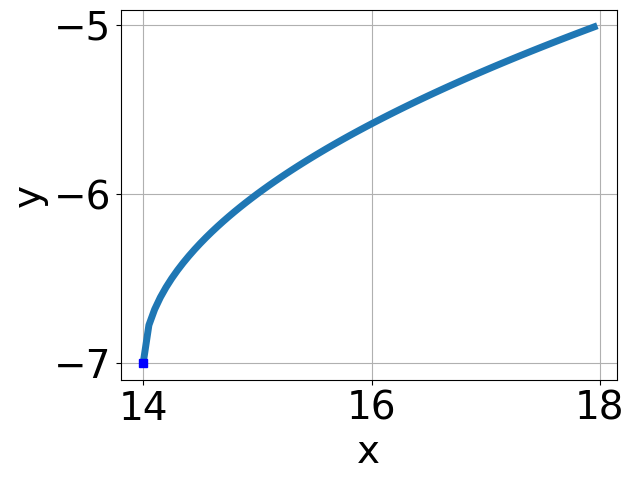
\includegraphics[width = 0.3\textwidth]{../Figures/radicalEquationToGraphCopyCA.png}\item 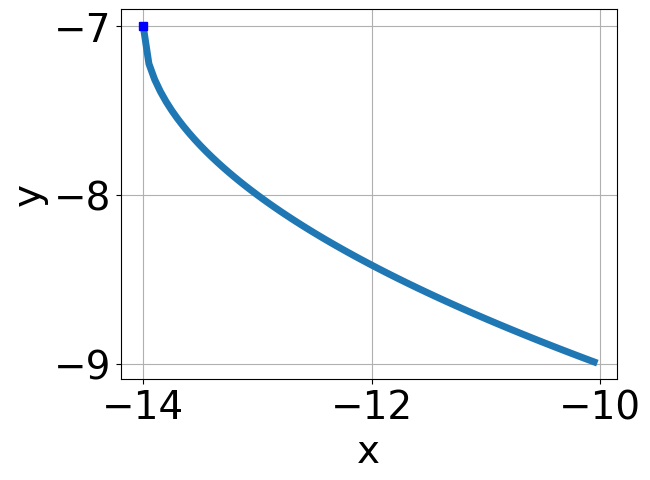
\includegraphics[width = 0.3\textwidth]{../Figures/radicalEquationToGraphCopyDA.png}\end{multicols}\item None of the above.
\end{enumerate} }
\litem{
What is the domain of the function below?\[ f(x) = \sqrt[5]{-9 x - 6} \]\begin{enumerate}[label=\Alph*.]
\item \( \text{The domain is } [a, \infty), \text{   where } a \in [-0.95, -0.02] \)
\item \( \text{The domain is } (-\infty, a], \text{   where } a \in [-1.7, -0.82] \)
\item \( \text{The domain is } [a, \infty), \text{   where } a \in [-1.73, -0.78] \)
\item \( \text{The domain is } (-\infty, a], \text{   where } a \in [-1.03, -0.19] \)
\item \( (-\infty, \infty) \)

\end{enumerate} }
\litem{
Solve the radical equation below. Then, choose the interval(s) that the solution(s) belongs to.\[ \sqrt{-6 x + 5} - \sqrt{8 x + 8} = 0 \]\begin{enumerate}[label=\Alph*.]
\item \( x_1 \in [-1.15, -0.55] \text{ and } x_2 \in [-1.17,1.83] \)
\item \( x \in [-0.31,0.77] \)
\item \( \text{All solutions lead to invalid or complex values in the equation.} \)
\item \( x_1 \in [-0.31, 0.77] \text{ and } x_2 \in [-1.17,1.83] \)
\item \( x \in [0.92,1.48] \)

\end{enumerate} }
\litem{
Choose the equation of the function graphed below.
\begin{center}
    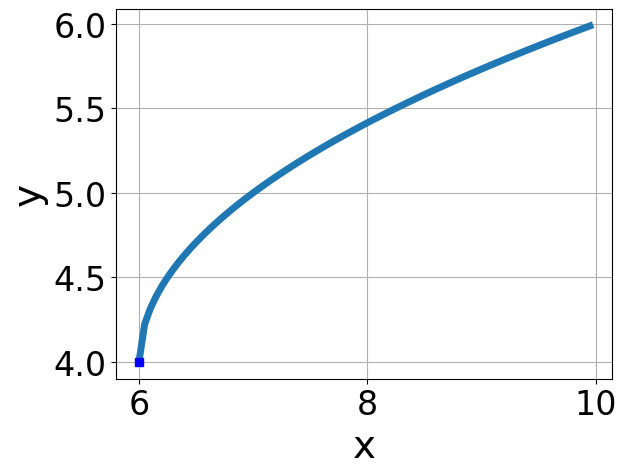
\includegraphics[width=0.5\textwidth]{../Figures/radicalGraphToEquationCopyB.png}
\end{center}
\begin{enumerate}[label=\Alph*.]
\item \( f(x) = \sqrt{x + 6} + 4 \)
\item \( f(x) = - \sqrt{x + 6} + 4 \)
\item \( f(x) = - \sqrt{x - 6} + 4 \)
\item \( f(x) = \sqrt{x - 6} + 4 \)
\item \( \text{None of the above} \)

\end{enumerate} }
\litem{
Choose the graph of the equation below.\[ f(x) = - \sqrt{x - 8} + 3 \]\begin{enumerate}[label=\Alph*.]
\begin{multicols}{2}\item 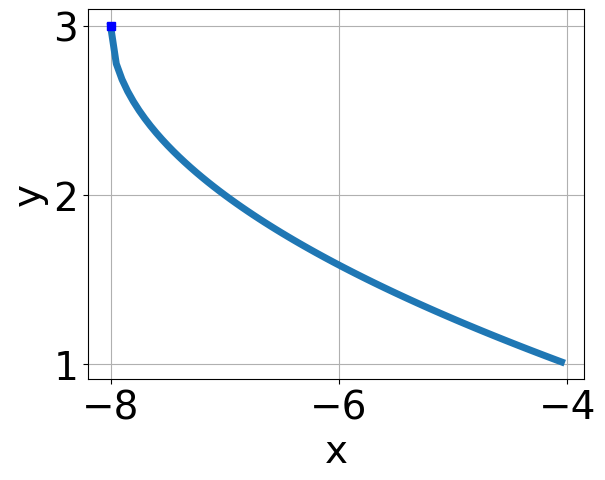
\includegraphics[width = 0.3\textwidth]{../Figures/radicalEquationToGraphAB.png}\item 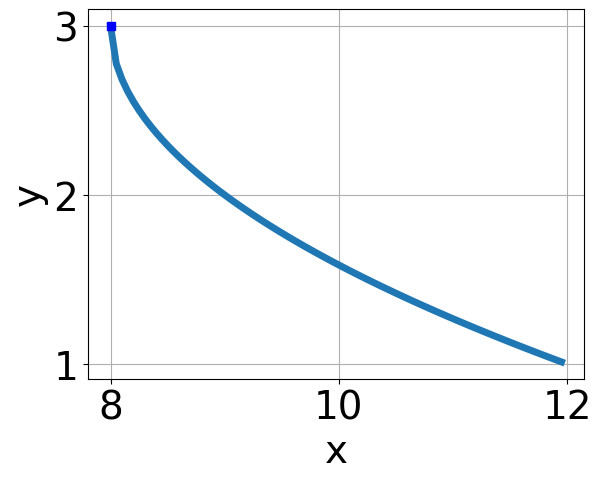
\includegraphics[width = 0.3\textwidth]{../Figures/radicalEquationToGraphBB.png}\item 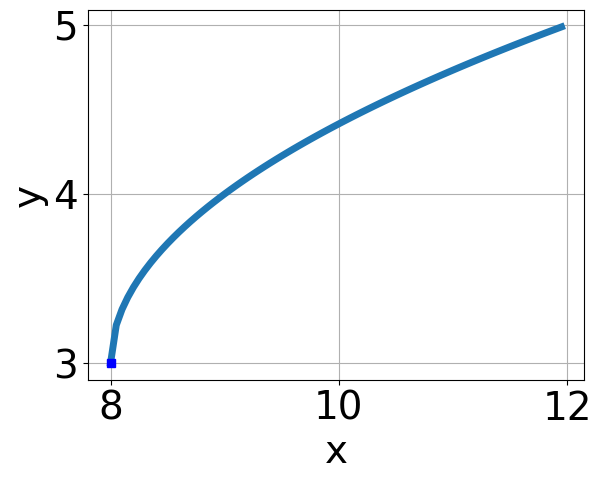
\includegraphics[width = 0.3\textwidth]{../Figures/radicalEquationToGraphCB.png}\item 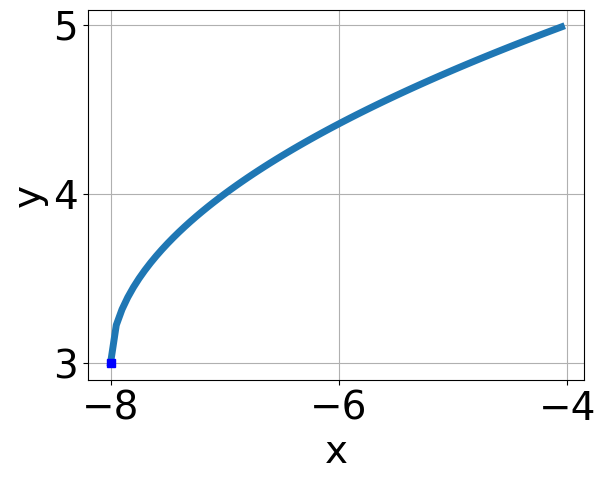
\includegraphics[width = 0.3\textwidth]{../Figures/radicalEquationToGraphDB.png}\end{multicols}\item None of the above.
\end{enumerate} }
\litem{
Solve the radical equation below. Then, choose the interval(s) that the solution(s) belongs to.\[ \sqrt{63 x^2 + 10} - \sqrt{59 x} = 0 \]\begin{enumerate}[label=\Alph*.]
\item \( x_1 \in [-0.44, 0.67] \text{ and } x_2 \in [0.6,2.1] \)
\item \( x_1 \in [-0.88, -0.67] \text{ and } x_2 \in [-0.6,-0.1] \)
\item \( x \in [0.27,1.08] \)
\item \( \text{All solutions lead to invalid or complex values in the equation.} \)
\item \( x \in [-0.44,0.67] \)

\end{enumerate} }
\litem{
Choose the equation of the function graphed below.
\begin{center}
    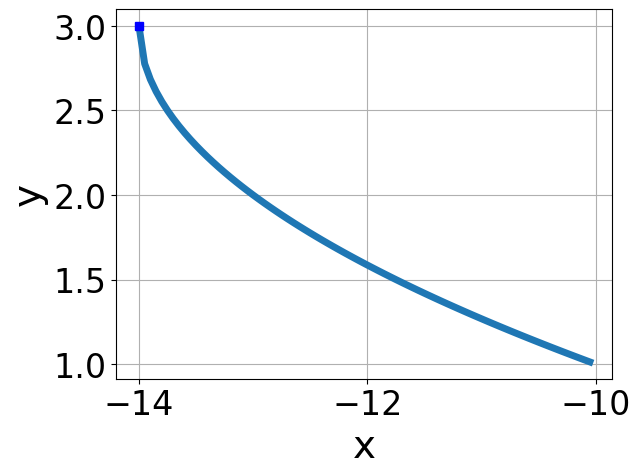
\includegraphics[width=0.5\textwidth]{../Figures/radicalGraphToEquationB.png}
\end{center}
\begin{enumerate}[label=\Alph*.]
\item \( f(x) = \sqrt{x + 14} + 3 \)
\item \( f(x) = - \sqrt{x - 14} + 3 \)
\item \( f(x) = \sqrt{x - 14} + 3 \)
\item \( f(x) = - \sqrt{x + 14} + 3 \)
\item \( \text{None of the above} \)

\end{enumerate} }
\litem{
Solve the radical equation below. Then, choose the interval(s) that the solution(s) belongs to.\[ \sqrt{-12 x^2 + 30} - \sqrt{-2 x} = 0 \]\begin{enumerate}[label=\Alph*.]
\item \( x_1 \in [1.3, 1.55] \text{ and } x_2 \in [-3.33,2.67] \)
\item \( x_1 \in [-1.64, -1.4] \text{ and } x_2 \in [-3.33,2.67] \)
\item \( \text{All solutions lead to invalid or complex values in the equation.} \)
\item \( x \in [-1.64,-1.4] \)
\item \( x \in [1.6,1.77] \)

\end{enumerate} }
\litem{
Solve the radical equation below. Then, choose the interval(s) that the solution(s) belongs to.\[ \sqrt{-4 x + 8} - \sqrt{-9 x - 6} = 0 \]\begin{enumerate}[label=\Alph*.]
\item \( x_1 \in [-1.21, -0.61] \text{ and } x_2 \in [-2,7] \)
\item \( x_1 \in [-3.15, -2.55] \text{ and } x_2 \in [-2,7] \)
\item \( x \in [-3.15,-2.55] \)
\item \( x \in [-0.45,0.32] \)
\item \( \text{All solutions lead to invalid or complex values in the equation.} \)

\end{enumerate} }
\litem{
What is the domain of the function below?\[ f(x) = \sqrt[5]{-6 x + 4} \]\begin{enumerate}[label=\Alph*.]
\item \( \text{The domain is } (-\infty, a], \text{   where } a \in [-5.2, 1.4] \)
\item \( \text{The domain is } (-\infty, a], \text{   where } a \in [1.2, 1.9] \)
\item \( (-\infty, \infty) \)
\item \( \text{The domain is } [a, \infty), \text{   where } a \in [1.32, 1.96] \)
\item \( \text{The domain is } [a, \infty), \text{   where } a \in [-0.15, 1.37] \)

\end{enumerate} }
\litem{
Choose the graph of the equation below.\[ f(x) = - \sqrt{x + 6} - 5 \]\begin{enumerate}[label=\Alph*.]
\begin{multicols}{2}\item 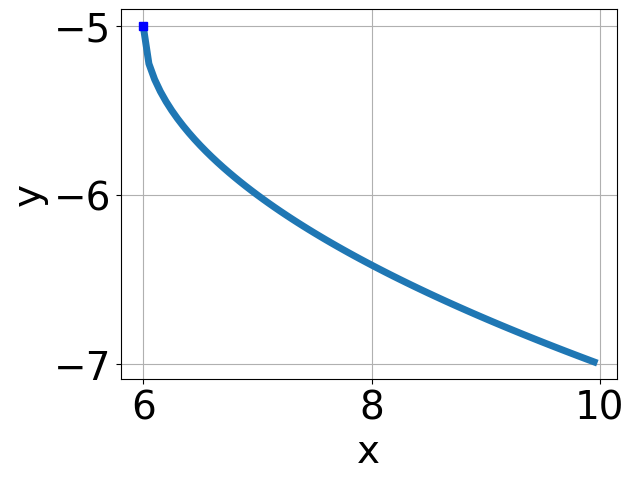
\includegraphics[width = 0.3\textwidth]{../Figures/radicalEquationToGraphCopyAB.png}\item 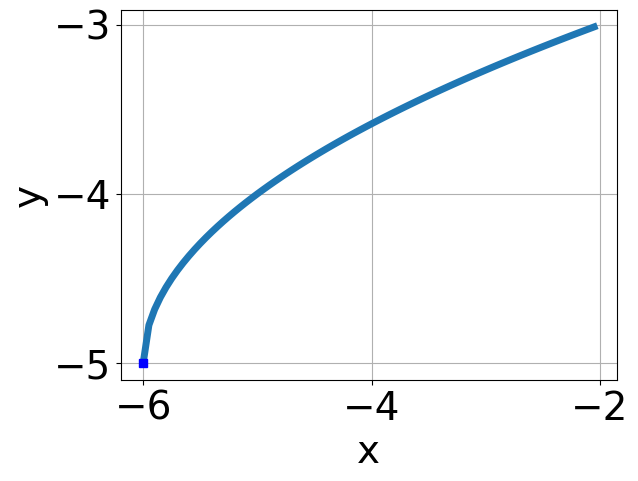
\includegraphics[width = 0.3\textwidth]{../Figures/radicalEquationToGraphCopyBB.png}\item 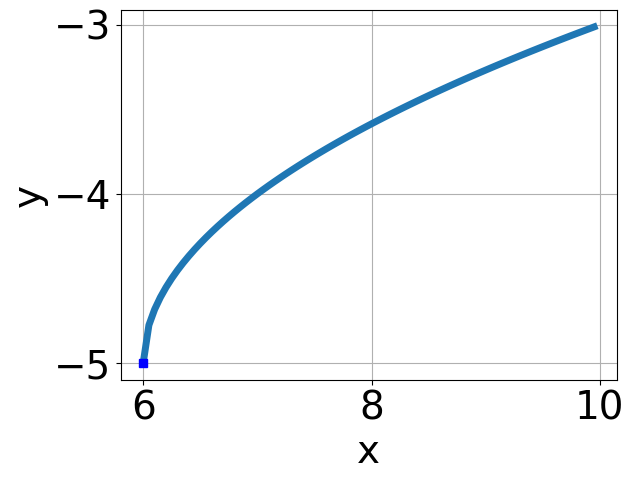
\includegraphics[width = 0.3\textwidth]{../Figures/radicalEquationToGraphCopyCB.png}\item 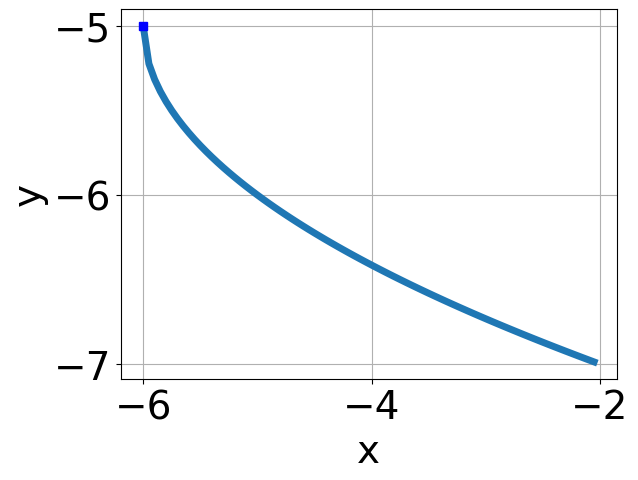
\includegraphics[width = 0.3\textwidth]{../Figures/radicalEquationToGraphCopyDB.png}\end{multicols}\item None of the above.
\end{enumerate} }
\litem{
What is the domain of the function below?\[ f(x) = \sqrt[6]{3 x + 6} \]\begin{enumerate}[label=\Alph*.]
\item \( [a, \infty), \text{where } a \in [-0.6, 0.2] \)
\item \( (-\infty, a], \text{where } a \in [-2.3, -1.5] \)
\item \( (-\infty, a], \text{where } a \in [-1.8, 0.5] \)
\item \( (-\infty, \infty) \)
\item \( [a, \infty), \text{ where } a \in [-2.8, -0.7] \)

\end{enumerate} }
\litem{
Solve the radical equation below. Then, choose the interval(s) that the solution(s) belongs to.\[ \sqrt{7 x + 6} - \sqrt{9 x - 9} = 0 \]\begin{enumerate}[label=\Alph*.]
\item \( x \in [7.22,8.19] \)
\item \( x_1 \in [-1.3, 0.85] \text{ and } x_2 \in [-1,4] \)
\item \( x_1 \in [-1.3, 0.85] \text{ and } x_2 \in [5.5,11.5] \)
\item \( \text{All solutions lead to invalid or complex values in the equation.} \)
\item \( x \in [-3.06,-0.9] \)

\end{enumerate} }
\litem{
Choose the equation of the function graphed below.
\begin{center}
    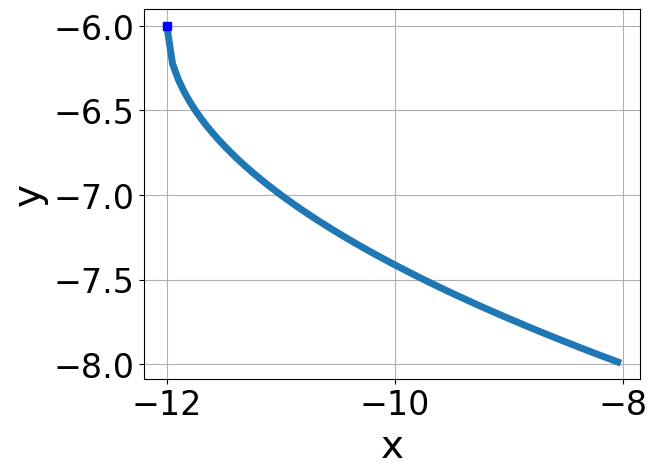
\includegraphics[width=0.5\textwidth]{../Figures/radicalGraphToEquationCopyC.png}
\end{center}
\begin{enumerate}[label=\Alph*.]
\item \( f(x) = \sqrt{x - 12} - 6 \)
\item \( f(x) = - \sqrt{x - 12} - 6 \)
\item \( f(x) = \sqrt{x + 12} - 6 \)
\item \( f(x) = - \sqrt{x + 12} - 6 \)
\item \( \text{None of the above} \)

\end{enumerate} }
\litem{
Choose the graph of the equation below.\[ f(x) = - \sqrt[3]{x + 14} + 4 \]\begin{enumerate}[label=\Alph*.]
\begin{multicols}{2}\item 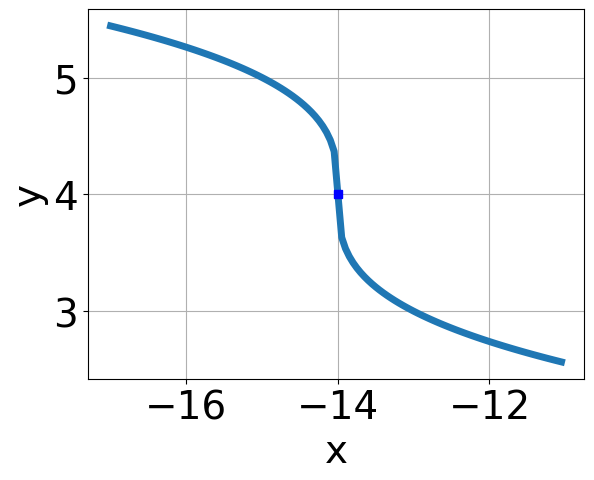
\includegraphics[width = 0.3\textwidth]{../Figures/radicalEquationToGraphAC.png}\item 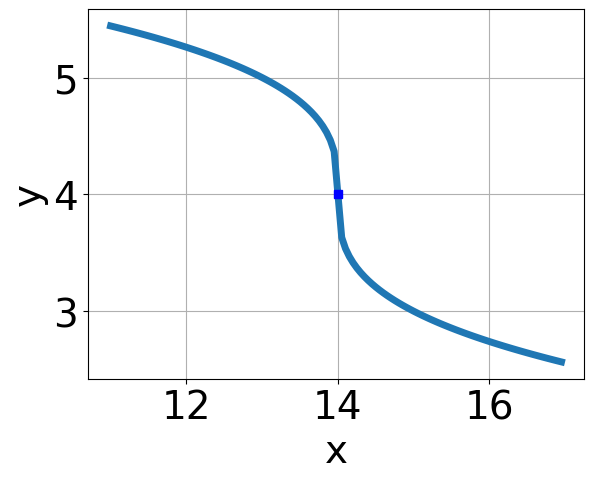
\includegraphics[width = 0.3\textwidth]{../Figures/radicalEquationToGraphBC.png}\item 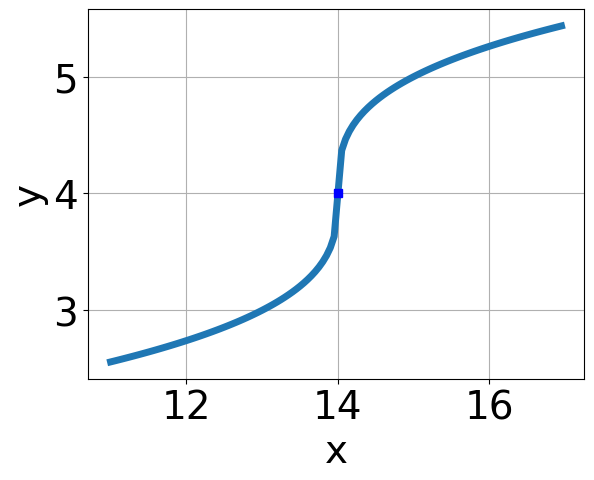
\includegraphics[width = 0.3\textwidth]{../Figures/radicalEquationToGraphCC.png}\item 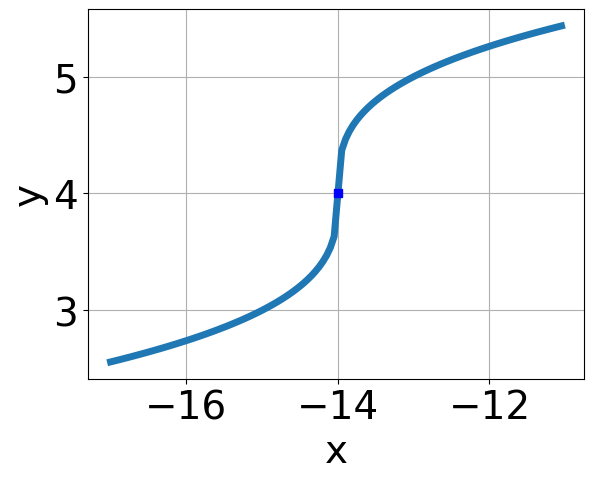
\includegraphics[width = 0.3\textwidth]{../Figures/radicalEquationToGraphDC.png}\end{multicols}\item None of the above.
\end{enumerate} }
\litem{
Solve the radical equation below. Then, choose the interval(s) that the solution(s) belongs to.\[ \sqrt{-40 x^2 + 8} - \sqrt{-4 x} = 0 \]\begin{enumerate}[label=\Alph*.]
\item \( \text{All solutions lead to invalid or complex values in the equation.} \)
\item \( x \in [0.42,0.5] \)
\item \( x \in [-0.56,-0.3] \)
\item \( x_1 \in [-0.56, -0.3] \text{ and } x_2 \in [-5.5,4.5] \)
\item \( x_1 \in [0.35, 0.45] \text{ and } x_2 \in [-5.5,4.5] \)

\end{enumerate} }
\litem{
Choose the equation of the function graphed below.
\begin{center}
    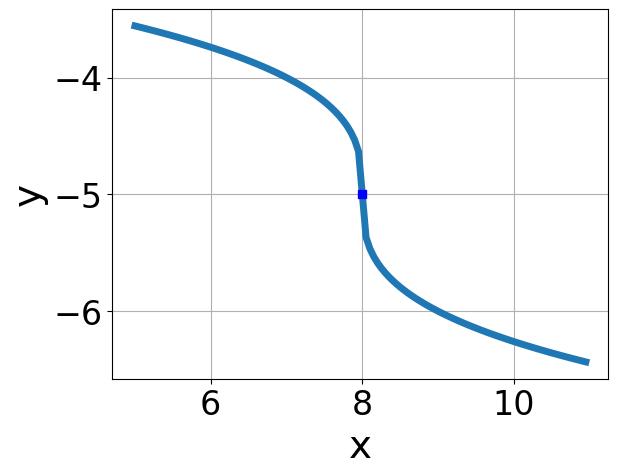
\includegraphics[width=0.5\textwidth]{../Figures/radicalGraphToEquationC.png}
\end{center}
\begin{enumerate}[label=\Alph*.]
\item \( f(x) = \sqrt[3]{x - 8} - 5 \)
\item \( f(x) = \sqrt[3]{x + 8} - 5 \)
\item \( f(x) = - \sqrt[3]{x - 8} - 5 \)
\item \( f(x) = - \sqrt[3]{x + 8} - 5 \)
\item \( \text{None of the above} \)

\end{enumerate} }
\litem{
Solve the radical equation below. Then, choose the interval(s) that the solution(s) belongs to.\[ \sqrt{10 x^2 + 45} - \sqrt{-55 x} = 0 \]\begin{enumerate}[label=\Alph*.]
\item \( \text{All solutions lead to invalid or complex values in the equation.} \)
\item \( x \in [-5.6,-3.1] \)
\item \( x \in [-1.1,0.1] \)
\item \( x_1 \in [-5.6, -3.1] \text{ and } x_2 \in [-4,1] \)
\item \( x_1 \in [0.2, 1.3] \text{ and } x_2 \in [0.5,6.5] \)

\end{enumerate} }
\litem{
Solve the radical equation below. Then, choose the interval(s) that the solution(s) belongs to.\[ \sqrt{-4 x - 8} - \sqrt{5 x - 6} = 0 \]\begin{enumerate}[label=\Alph*.]
\item \( x \in [-0.92,1.18] \)
\item \( x_1 \in [-2.87, -1.88] \text{ and } x_2 \in [1,2.4] \)
\item \( x \in [-1.86,-1.48] \)
\item \( \text{All solutions lead to invalid or complex values in the equation.} \)
\item \( x_1 \in [-2.87, -1.88] \text{ and } x_2 \in [-0.9,0.9] \)

\end{enumerate} }
\litem{
What is the domain of the function below?\[ f(x) = \sqrt[4]{-5 x + 8} \]\begin{enumerate}[label=\Alph*.]
\item \( [a, \infty), \text{where } a \in [0, 1] \)
\item \( (-\infty, a], \text{where } a \in [-1.3, 1.2] \)
\item \( (-\infty, \infty) \)
\item \( (-\infty, a], \text{ where } a \in [1.3, 5.9] \)
\item \( [a, \infty), \text{where } a \in [1.1, 4.5] \)

\end{enumerate} }
\litem{
Choose the graph of the equation below.\[ f(x) = \sqrt{x - 10} + 7 \]\begin{enumerate}[label=\Alph*.]
\begin{multicols}{2}\item 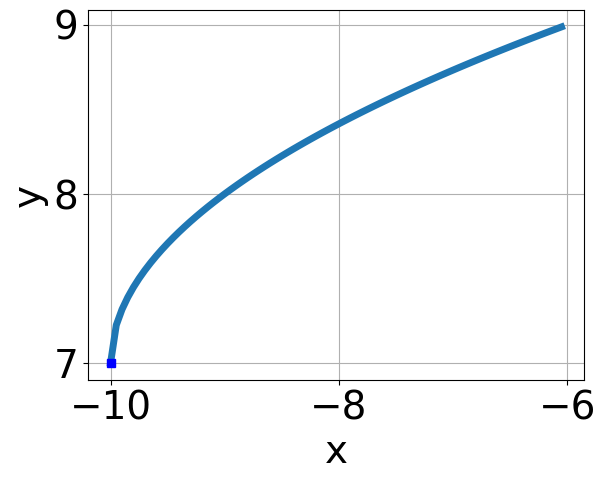
\includegraphics[width = 0.3\textwidth]{../Figures/radicalEquationToGraphCopyAC.png}\item 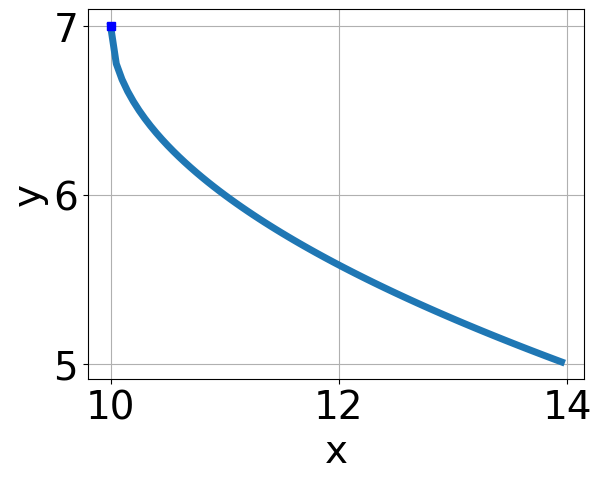
\includegraphics[width = 0.3\textwidth]{../Figures/radicalEquationToGraphCopyBC.png}\item 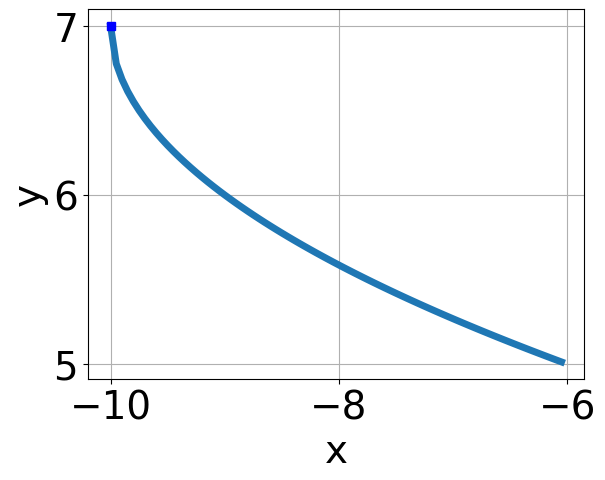
\includegraphics[width = 0.3\textwidth]{../Figures/radicalEquationToGraphCopyCC.png}\item 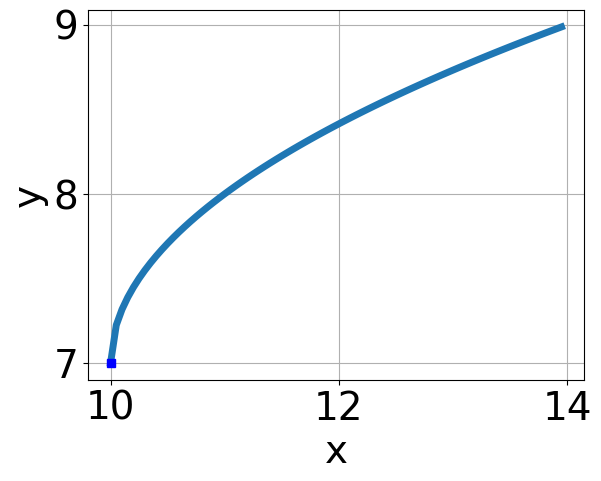
\includegraphics[width = 0.3\textwidth]{../Figures/radicalEquationToGraphCopyDC.png}\end{multicols}\item None of the above.
\end{enumerate} }
\litem{
What is the domain of the function below?\[ f(x) = \sqrt[5]{3 x - 9} \]\begin{enumerate}[label=\Alph*.]
\item \( \text{The domain is } [a, \infty), \text{   where } a \in [0.3, 1.6] \)
\item \( \text{The domain is } (-\infty, a], \text{   where } a \in [-1.67, 2.33] \)
\item \( \text{The domain is } [a, \infty), \text{   where } a \in [1.6, 6.1] \)
\item \( (-\infty, \infty) \)
\item \( \text{The domain is } (-\infty, a], \text{   where } a \in [2, 5] \)

\end{enumerate} }
\litem{
Solve the radical equation below. Then, choose the interval(s) that the solution(s) belongs to.\[ \sqrt{9 x + 8} - \sqrt{7 x + 2} = 0 \]\begin{enumerate}[label=\Alph*.]
\item \( x_1 \in [-3.06, -2.66] \text{ and } x_2 \in [-1.29,-0.58] \)
\item \( x \in [-3.06,-2.66] \)
\item \( x \in [-5.14,-3.53] \)
\item \( \text{All solutions lead to invalid or complex values in the equation.} \)
\item \( x_1 \in [-1.31, 0.27] \text{ and } x_2 \in [-0.54,0.15] \)

\end{enumerate} }
\end{enumerate}

\end{document}